\documentclass{article}
\usepackage[utf8]{inputenc}
\usepackage[spanish,mexico,es-lcroman]{babel}
\usepackage{enumitem}
\usepackage{amssymb}
\usepackage{listingsutf8}
\usepackage{amsmath}
\usepackage{geometry}
\usepackage[outline]{contour}
\usepackage[dvipsnames]{xcolor}
\geometry{tmargin=2cm, lmargin=2.5cm, rmargin=2.5cm, bmargin=2cm}
\usepackage{tikz}
\usepackage{xcolor}

\usepackage{blindtext}

\usepackage{hyperref}

\hypersetup{
    colorlinks=true,
    linkcolor=blue,
    filecolor=magenta,      
    urlcolor=cyan,
    }

\lstset{
    inputencoding=utf8,
    extendedchars=true,
    literate={á}{{\'a}}1 {é}{{\'e}}1 {í}{{\'i}}1 {ó}{{\'o}}1 {ú}{{\'u}}1 {ñ}{{\~n}}1
}
    
\urlstyle{same}

\definecolor{codegreen}{rgb}{0,0.6,0}
\definecolor{codegray}{rgb}{0.5,0.5,0.5}
\definecolor{codepurple}{rgb}{0.58,0,0.82}
\definecolor{backcolour}{rgb}{0.95,0.95,0.92}

\lstdefinestyle{mystyle}{
  backgroundcolor=\color{backcolour}, commentstyle=\color{codegreen},
  keywordstyle=\color{magenta},
  numberstyle=\tiny\color{codegray},
  stringstyle=\color{codepurple},
  basicstyle=\ttfamily\footnotesize,
  breakatwhitespace=false,         
  breaklines=true,                 
  captionpos=b,                    
  keepspaces=true,                 
  numbers=left,                    
  numbersep=5pt,                  
  showspaces=false,                
  showstringspaces=false,
  showtabs=false,                  
  tabsize=2
}
\lstset{style=mystyle}



\begin{document}

\section*{Introducción}

En esta práctia veremos el funcionamiento y como implementar curvas elípticas para el cifrado y descifrado de mensaje, el uso del protocolo Diffie-Hellman, se verán ejemplos del funcionamiento para entender el proceso de creación y manejo de llaves públicas y privadas entre las entidades es decir como realizan el intercambio de llaves, la comparativa entre este nuevo como de cifrado en comparación con RSA, y el nivel de seguridad que tiene ante ataques.

\section*{Desarrollo.}

El archivo diferencial se adjuntara junto con el pdf, a continuación se muestra que el código pasa todas las pruebas:

\begin{center}
    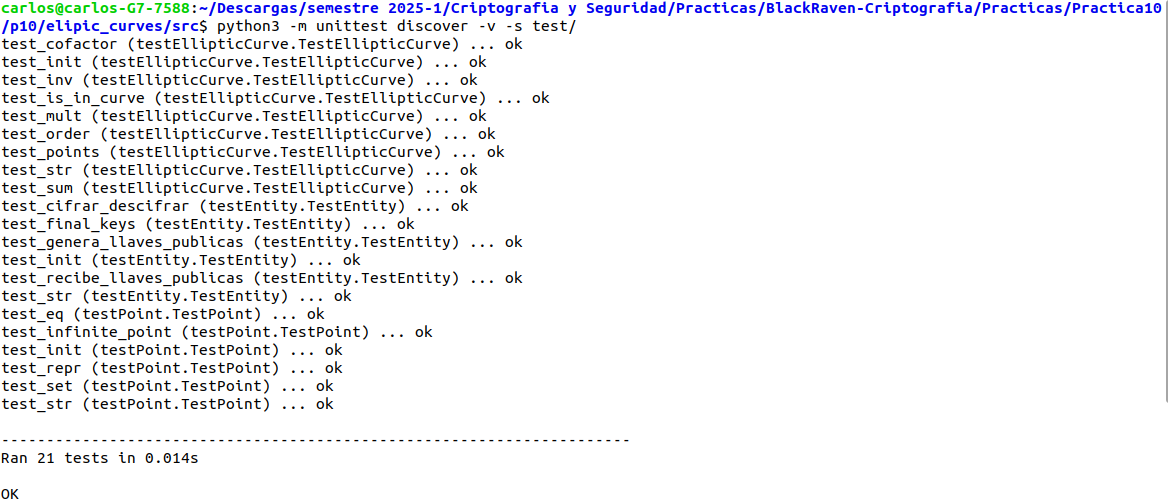
\includegraphics[scale = .45]{IMAGE/Pruebas.png}
\end{center}

\section*{Preguntas}

Contesta las siguiente preguntas, investigando o con tus propias palabras.

\begin{enumerate}

    \item Cuando sumamos un punto P con -P , que nos da como resultado el punto al infinito... ¿Qué quiere decir que un punto sea infinito?

    En las curvas elípticas,cuando nos referimos "punto al infinito" (denotado como O) es un concepto matemático abstracto.

    Cuando hablamos del punto al infinito en curvas elípticas, no nos referimos a un punto que está "muy lejos" en el sentido usual, es al algo más que eso.

    Puede actuar como un elemento neutro en la operación de grupo de la curva elíptica. Esto significa que, para cualquier punto P en la curva:
    \begin{itemize}
        \item P + O = P (para cualquier punto P)

        \item O + P = P

        \item P + (-P) = O

        \item O + O = O
    \end{itemize}
    
    Geométricamente, cuando sumamos P y -P, la línea que une estos puntos es vertical, esta línea ''interseca'' la curva en el punto al infinito, es como si continuara hacia arriba indefinidamente, Esto sucede porque -P es el reflejo de P respecto al eje x, y cuando los sumamos, las tangentes a la curva se anulan, proyectándose fuera de cualquier coordenada finita.

    \item Cuando sumamos un punto P consigo mismo, ¿qué característica tiene la recta que conecta a estos 2 puntos?

    Esta respuesta nos basamos en el link que se puede encontrar en referencias del pdf \textbf{Ataques de Tiempo a Rutinas Criptográficas sobre Curvas Elípticas, pag. 18 capítulo 3}

    Si P y Q son el mismo punto, la línea recta que los conecta sera una tangente a la curva en ese punto. Para obtener el punto de intersección R, simplemente reflejas el punto de interseccion sobre el eje x. 

    Si sumamos dos veces P lo que estamos obteniendo es una duplicación de puntos, para este caso la recta es la tangente a la curva elíptica en el punto P.

    Esta tangente es única para cada punto P, la recta que ''toca'' la curva en un solo punto (el punto P), además representa la "pendiente instantánea" de la curva en ese punto.

    Para encontrar esta pendiente de la línea tangente se calcula usando la derivada de la ecuación de la curva en el punto P, la recta intersecará la curva en otro punto y el reflejo de este punto de intersección sobre el eje x será 2P

    \item ¿En qué otro cifrado se utiliza el protoclo Diffie-Hellman?. 

    El intercambio de claves Diffie-Hellman se puede utilizar para establecer claves públicas y privadas. Sin embargo, en la práctica, se tiende a utilizar RSA en su lugar. Esto se debe a que el algoritmo RSA también es capaz de firmar certificados de clave pública, mientras que el intercambio de claves Diffie-Hellman no lo es.

    El algoritmo ElGamal, que se usó mucho en PGP, se basa en el intercambio de claves Diffie-Hellman, por lo que cualquier protocolo que lo use está implementando efectivamente una especie de Diffie-Hellman.

    Como uno de los métodos más comunes para distribuir claves de forma segura, el intercambio de claves Diffie-Hellman se implementa con frecuencia en protocolos de seguridad como:

    \begin{itemize}
        \item SSL (Secure Socket Layer)

        \item TLS (Transport Layer Security)

        \item IPsec

        \item SSH (Secure Shell)

        \item VPN (Virtual Private Network)

        \item PGP

        \item Tor
        
        \item Off-the-Record Messaging (OTR)
    \end{itemize}

    y muchos otros. Esto lo convierte en una parte integral de nuestras comunicaciones seguras.

    \item ¿Cuántos bits de una llave de una curva necesitamos para poder igualar la seguridad en una llave de RSA?

    Para poder igualar la seguridad de una llave RSA, las curvas elípticas necesitan de una cantidad de bits relativamente menor esto de debe a su eficiencia en seguridad, entonces tenemos lo siguiente de curva elíptica vs RSA:

    \begin{itemize}
        \item 224 bits $\equiv$ 2048 bits

        \item 256 bits $\equiv$ 3072 bits

        \item 384 bits $\equiv$ 7680 bits

        \item 512 bits $\equiv$ 15360 bits
    \end{itemize}

    \item En el ejemplo, en attack tenemos que la letra 't' es cifrada a 2 puntos diferentes de la curva, y sigue siendo recuperable. ¿qué valor hace esto posible?

    El caracter t puede ser mapeado a diferentes puntos de la curva, el valor que permite esta variabilidad es el uso de valores aleatorios cuando se cifra por eso el uso de random para Entity, este valor único se incluye en cada operación de cifrado y modifica el resultado sin cambiar el mensaje descifrado, la clave privada puede recuperar el mensaje original independientemente del valor usado, por lo que es aqui que hace que el carácter se pueda cirfra de forma diferente. 

    \item Cifra el mensaje: Perro salchicha, gordo bachicha usando la curva elíptica $EC_{233}$(-2, 8) usando los 256 caracteres del código ASCCI. Pega la ejecución de la salida del main\\

    Tenemos lo siguiente:

    \begin{center}
        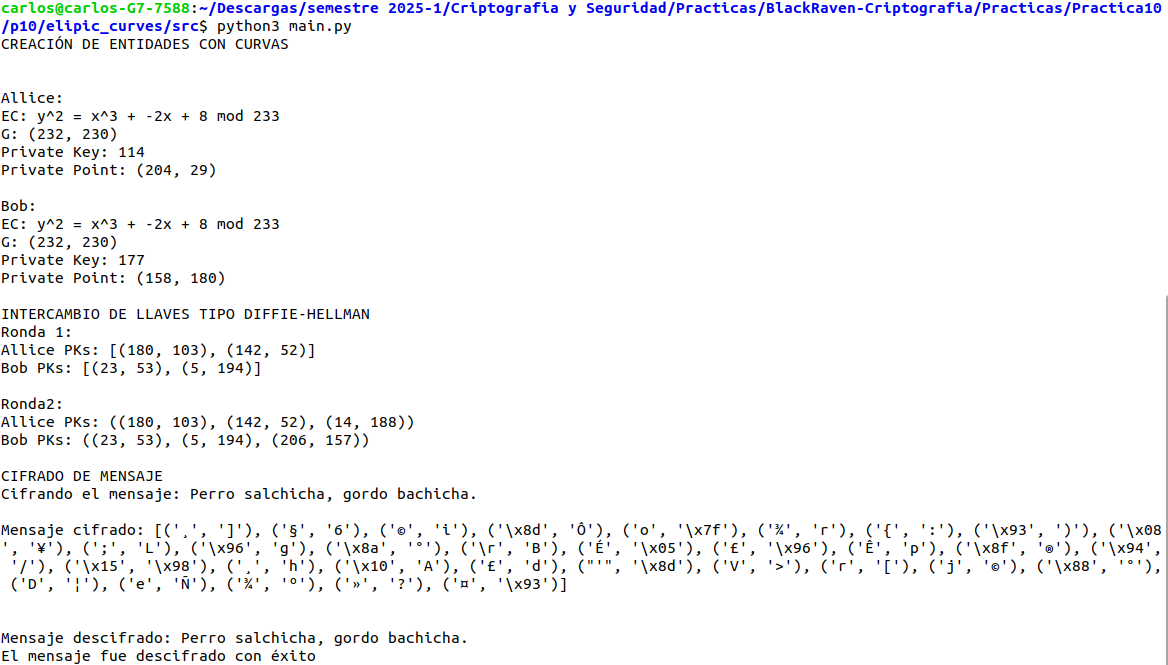
\includegraphics[scale = .41]{IMAGE/E6.png}
    \end{center}

    Podemos ver que el codigo funciona y cifra y descifra el mensaje correctamente.

\end{enumerate}

\section*{Conclusión}

\begin{enumerate}
    \item \textbf{Carlos}: El curso me gustó mucho siento que es impresindible conocer, aprender y saber como poder defenderse y como mantenerse seguro en el dia a dia en cuanto a la ciberseguridad, los temas y la estructura que tiene el curso me parece adecuada, pero a mi parecer falta tener más tiempo, ya que a veces por entregar las taeas o prácticas uno le interesa más entregar los trabajos, sin embargo considero que en cuanto a lo que se enseñó esta muy bien, también cabe recalcar de que al haber aprendido todo lo del curso debemos tener la ética y responsabilidad de no causar daño a otros con los conocimientos adquiridos.

    Otro punto a considerar diría es que se podría dar mas ejemplos os tutoriales como nuestro compañero comenta abajo, como lo fue el caso de la práctica 9 de servidores en la nube, que en mi caso si nos costó mucho trabajo y nos sentieamos perdidos continuamente, con respecto a lo demás no tengo más que añadir, diría que esta muy bien.

    En general dire que es un curso completo, que resulto ser de mi agrado pero muy estresante debido a los tiempos, muchas gracias por haber impartido esta materia.  

    \item \textbf{Jonathan}: El curso me gustó y es interesante todo lo que vimos, desde los algoritmos hasta los temas de ciberseguridad, de igual manera todo lo que se podía hacer simplemente buscando un poco en internet o preguntándole a la IA (en el caso de los malware), lo cuál nos deja con una responsabilidad de no usar lo aprendido para hacer algún daño. Quizá algo a mejorar podría ser un mejor tutorial al usar tecnologías que no se hayan usado antes, como fue el caso de los servicios en la nube. Si bien la ciberseguridad es importante y día a día se hacen avances respecto a esta, no creo profundizar más allá de leer por mera curiosidad.

    \item \textbf{Edgar}: El curso me pareció pesado pero entretenido, me gustaría haberla cursado con una menor cantidad de materias para poder dedicarle más tiempo, en lo personal no creo dedicarme a la ciberseguridad, aunque me pareció interesante pero adentrarse más a fondo requiere de mucha concentración, en lo que respecta al curso, me gustaria que dejen material complementario cuando se realizan las prácticas o tarea, compartó la idea de mis otros compañeros refiriendonos a la práctica 9 de servidores en la nube, me hubiera gustado tener una guía mas completa para poder haber abordado mejor ese tema.
\end{enumerate}

{\color{black}\rule{\textwidth}{1.5pt}}

\section*{Referencias}

\begin{itemize}

    \item Buurstra Parmo, G. (2023). Criptografía de curvas elípticas [Trabajo de Fin de Grado, Universidad Politécnica de Madrid]. Archivo Digital UPM. 

    \url{https://oa.upm.es/75495/1/TFG_GABRIELA_BUURSTRA_PARMO.pdf}

    \item Ciberseguridad.com. (s.f.). Intercambio de claves Diffie-Hellman.

    \url{https://ciberseguridad.com/guias/recursos/intercambio-claves-diffie-hellman/}

    \item  Diffie-Hellman key exchange. (2023). En Wikipedia.

    \url{https://es.wikipedia.org/wiki/Intercambio_de_claves_de_Diffie-Hellman}

    \item  Elliptic curve. (2023). En Wikipedia. 

    \url{https://es.wikipedia.org/wiki/Curva_el%C3%ADptica}

    \item  Elliptic-curve cryptography. (2023). En Wikipedia.

    \url{https://en.wikipedia.org/wiki/Elliptic-curve_cryptography}

    \item  Kolokium. (2023). Criptografía de curva elíptica.

    \url{https://kolokium.com/blog/criptografia-de-curva-eliptica/}

    \item  Elliptic Curves. (s.f.). En Brilliant.

    \url{https://brilliant.org/wiki/elliptic-curves/}
    
\end{itemize}

{\color{black}\rule{\textwidth}{1.5pt}}
\end{document}

